\documentclass[a4paper,ngerman]{scrartcl}

\usepackage[utf8]{inputenc}
\usepackage{amssymb,amsmath}

\usepackage[ngerman]{babel}
\usepackage{pdfpages}

\usepackage{graphicx}

\usepackage[protrusion=true,expansion=true]{microtype}

\usepackage{hyperref}
\usepackage{libertine}
\usepackage{tabto}

\setlength\parskip{\medskipamount}
\setlength\parindent{0pt}

\usepackage{geometry}
\geometry{tmargin=1.5cm,bmargin=2cm,lmargin=1.5cm,rmargin=1.5cm}

\pagestyle{empty}

\setlength{\fboxrule}{2pt}
\setlength{\fboxsep}{-3pt}

\newcommand{\drawHere}{%
  \begin{center}%
    \fbox{\parbox[c][0.9\textwidth]{0.9\textwidth}{\ }}%
  \end{center}}

\newcommand{\header}{%
  \begin{raggedleft}
  \tiny Universität Augsburg \\
  Tag der Mathematik 2015 \par
  \end{raggedleft}}

\begin{document}

\header

\begin{center}
  \Huge\bf
  Die Kochsche Schneeflocke
\end{center}

\vfill
\drawHere

\vfill
\Large

\renewcommand{\labelitemi}{$\bigstar$}

\begin{itemize}
  \item So konstruiert man die Kochsche Schneeflocke:

  \begin{center}
    \includegraphics[scale=0.5]{koch}
  \end{center}
  \item Was ist ihr Umfang?
  \item Was ist ihr Flächeninhalt?
\end{itemize}

\newpage



\header

\begin{center}
  \Huge\bf
  Das Pascalsche Dreieck
\end{center}

\begin{center}
\includegraphics[scale=1.2]{pascal-triangle}
\end{center}

\renewcommand{\labelitemi}{$\triangle$}

\Large
\begin{itemize}
\item Fülle das Dreieck aus. Trage dazu überall am Rand den Wert $1$ ein. Der
Wert jedes Kästchens ergibt sich dann als Summe der beiden Kästchen darüber.
\item Die \emph{Dreieckszahlen} werden gebildet, indem man natürliche Zahlen
aufsummiert: Die erste Dreieckszahl ist $1$, danach kommt $1+2 = 3$, dann
$1+2+3 = 6$ und so weiter. Berechne doch mal die ersten acht Dreieckszahlen!
\begin{center}
% Quelle: http://www.cs4fn.org/algorithms/images/triangular.jpg
\includegraphics[scale=0.5]{triangular-numbers}
\end{center}
\item Kannst du die Dreieckszahlen im Pascalschen Dreieck entdecken? Wenn ja, wo?
\emph{Kannst du erklären, wieso sie dort auftreten?}
\item Male alle Felder mit ungeraden Zahlen im Pascalschen Dreieck aus. Kannst
du ein Muster erkennen?          
\end{itemize}

% Auf der Rückseite (für zu Hause): Fibonacci-Zahlen erkennen

\newpage

Am Pascalschen Dreieck gibt es noch viel mehr zu entdecken.

\begin{itemize}
\item Addiert man die Zahlen auf den einzelnen Zeilen des Pascalschen Dreiecks,
so erhält man die \emph{Zweier-Potenzen}: $1, 2, 4, 8, 16, \ldots$

\item Kennst du schon die \emph{binomische Formel}~$(x+y)^2 = x^2 + 2xy + y^2$?
Wolltest du schon immer wissen, wie man ähnlich flott~$(x+y)^3$, $(x+y)^4$ und
so weiter ausrechnen kann, ohne ewig die Klammern ausmultiplizieren zu müssen?
Mit dem Pascalschen Dreieck geht das ganz einfach:
\begin{align*}
  (x+y)^3 &= x^3 + 3x^2y + 3xy^2 + y^3 \\
  (x+y)^4 &= x^4 + 4x^3y + 6x^2y^2 + 4xy^3 + y^4 \\
  (x+y)^5 &= x^5 + 5x^4y + 10x^3y^2 + 10x^2y^3 + 5xy^4 + y^5
\end{align*}

\item Addiert man die Zahlen des Pascalschen Dreiecks wie in der Skizze auf, so
erhält man die \emph{Fibonacci-Zahlen}! Das ist die Folge der Zahlen
\[ 1, \quad 1, \quad 2, \quad 3, \quad 5, \quad 8, \quad 13, \quad 21, \quad
\ldots, \]
die nächste Zahl ist also immer die Summe der beiden vorhergehenden Zahlen.
Fibonacci-Zahlen kommen in der Natur sehr oft vor, zum Beispiel bei
Tannenzapfen und Sonnenblumen. Informiere dich doch bei Wikipedia darüber!

\begin{center}
% Quelle: http://www.geocities.ws/millers_math/famous/fiban.gif
\includegraphics[scale=0.9]{pascal-fibonacci}
\end{center}
\end{itemize}

\newpage




\header

\begin{center}
  \Huge\bf
  Das Sierpinski-Dreieck
\end{center}

\vfill
\drawHere

\vfill
\Large

\renewcommand{\labelitemi}{$\blacktriangle$}

\begin{itemize}
  \item Spiele folgendes \emph{Chaosspiel}:
  \begin{enumerate}
    \item Zeichne ein großes gleichseitiges Dreieck.
    \item Wähle einen beliebigen Startpunkt im Dreieck.
    \item Such dir zufällig eine der drei Ecken aus.
    \item Markiere als neuen Punkt die Mitte zwischen deiner gewählten Ecke und \\ dem
    vorherigen Punkt.
    \item Fahre mit dem neuen Punkt bei Schritt 3 fort.
  \end{enumerate}
\end{itemize}

\begin{itemize}
  \item Obwohl man den Startpunkt und die Ecken völlig zufällig wählt, ergibt
  sich erstaunlicherweise näherungsweise eine regelmäßige Figur: das \emph{Sierpinski-Dreieck}.
  \item Deterministisch (ohne Zufall) kann man es auch so konstruieren:

  \begin{center}
    \includegraphics[scale=0.1]{sierpinski-1}\hfill
    \includegraphics[scale=0.1]{sierpinski-2}\hfill
    \includegraphics[scale=0.1]{sierpinski-3}\hfill
    \includegraphics[scale=0.1]{sierpinski-4}
  \end{center}
  \item Wieso ergibt sich beim Chaosspiel dieses Sierpinski-Dreieck?

  Der Abstand der Punkte beim Chaosspiel zum tatsächlichen, völlig regelmäßigen
  Sierpinski-Dreieck halbiert sich mit jedem Schritt. Für das bloße Auge liegen
  daher alle Punkte (bis auf einige wenige zu Beginn) auf dem
  Sierpinski-Dreieck. Durch die zufällige Eckenwahl wird das ganze Dreieck
  gleichmäßig gefüllt.
  
  \begin{center}
    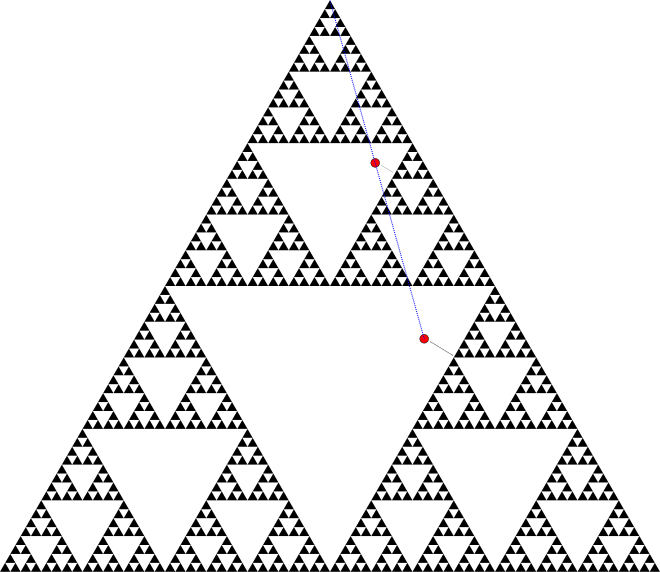
\includegraphics[scale=0.45]{sierpinski-beweis}
  \end{center}
  \item Was ist der Umfang des Sierpinski-Dreiecks?
  \item Was ist der Flächeninhalt des Sierpinski-Dreiecks?
  \item Die Kochsche Schneeflocke und das Sierpinski-Dreieck sind Beispiele für
  sog. \emph{Fraktale} (von lateinisch \emph{fractus}, "`gebrochen"').
  Annäherungen an Fraktale findet man an vielen Stellen in der Natur,
  etwa beim Romanesco-Blumenkohl, bei Flusssystemen, beim Blutkreislauf und bei
  Küstenlinien; außerdem sind manche physikalische Diagramme von fraktaler
  Natur.

  Fraktale sind
  wichtig, um sich klarzumachen, wie wunderlich geometrische Figuren sein
  können, und haben auch noch einen praktischen Nutzen: Fraktale werden
  in der Computergrafik eingesetzt, um realistisch aussehende Wälder und
  Wolken automatisiert
  generieren zu können.
\end{itemize}

\vfill
\hfill\small Chaosspiel direkt auf \url{http://tiny.cc/chaosspiel} spielbar

\end{document}
